\section{Milestone}
This section outlines the key milestones for the successful completion of the project, along with their respective timelines. The milestones are divided into distinct phases to ensure clarity and manageability throughout the project lifecycle.

\subsection{Project Milestones and Timeline}
The major milestones for the project are as follows:
\begin{enumerate}
    \item \textbf{Planning and Preparation (Week 1-3):}
    \begin{itemize}
        \item Define objectives, scope, and deliverables.
        \item Gather image datasets requirements.
        \item Finalize workflow and timeline.
    \end{itemize}
    
    \item \textbf{Data Collection and Preparation (Week 4-7):}
    \begin{itemize}
        \item Collect datasets of relevant images.
        \item Preprocess the data by cleaning and augmenting it.
        \item Split datasets into training and testing sets.
    \end{itemize}
    
    \item \textbf{Model Selection and Development (Week 8-10):}
    \begin{itemize}
        \item Research and select an appropriate image classification model.
        \item Design and implement the system architecture.
        \item Split the test data and train data for the selected model.
    \end{itemize}
    
    \item \textbf{Model Training and Tuning (Week 11-14):}
    \begin{itemize}
        \item Train the model using the prepared datasets.
        \item Tune hyperparameters to optimize performance.
        \item Evaluate the model using metrics such as accuracy, precision, and F1 score.
        \item Fine-tune the model based on evaluation results.
    \end{itemize}
    
    \item \textbf{Testing and Integration (Week 15-16):}
    \begin{itemize}
        \item Test the model for accuracy and usability.
        \item Integrate the model for real-time predictions.
    \end{itemize}
    
    \item \textbf{Documentation and Deployment (Week 17-18):}
    \begin{itemize}
        \item Prepare detailed documentation and reports.
        \item Create a presentation showcasing project progress and results.
        \item Deploy the model and application for end-user accessibility.
    \end{itemize}
\end{enumerate}


\subsection{Visualization of Timeline}
The timeline and schedule feasibility for the project phases are depicted in the Gantt chart below (Figure~\ref{fig:gantt-chart}).

\begin{figure}[H]
    \centering
    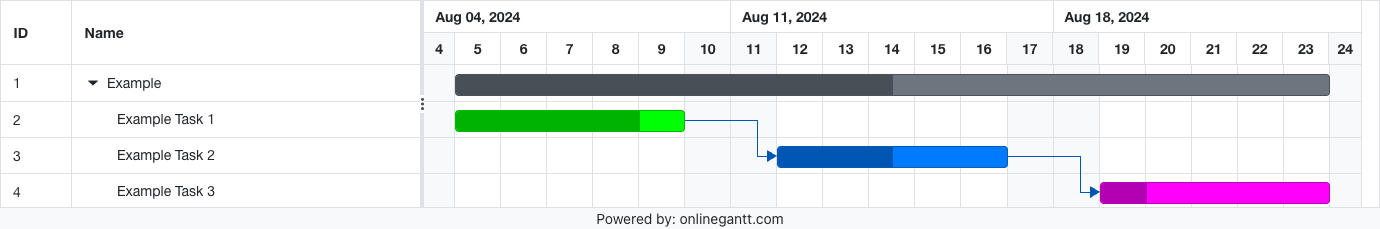
\includegraphics[width=1\linewidth]{Images/gantt.png}
    \caption{Sample Gantt Chart demonstrating schedule feasibility}
    \label{fig:gantt-chart}
\end{figure}
